%
%  Wakefield Acceleration
% ========================
%

\chapter{A Wakefield Accelerator Experiment}
\label{Ch:WFA}

AWAKE is the first proton driven wakefield accelerator experiment in the world. It is a proof-of-concept experiment aiming to inform a design for future high energy accelerators \cite{gschwendtner:2016}. The proton drive beam is delivered by the Super Proton Synchrotron (SPS) at CERN. The experiment is physically located at the former site of the CERN Neutrinos to Gran Sasso experiment (CNGS) \cite{gschwendtner:2010} in a tunnel below the Swiss-French border connected to the SPS at SPS Point 4. The placement of the AWAKE experiment in relation to the rest of the CERN accelerator complex can be seen in Figure \ref{Fig:WFA:AccComp}.

\begin{figure}[hbt]
    \centering
    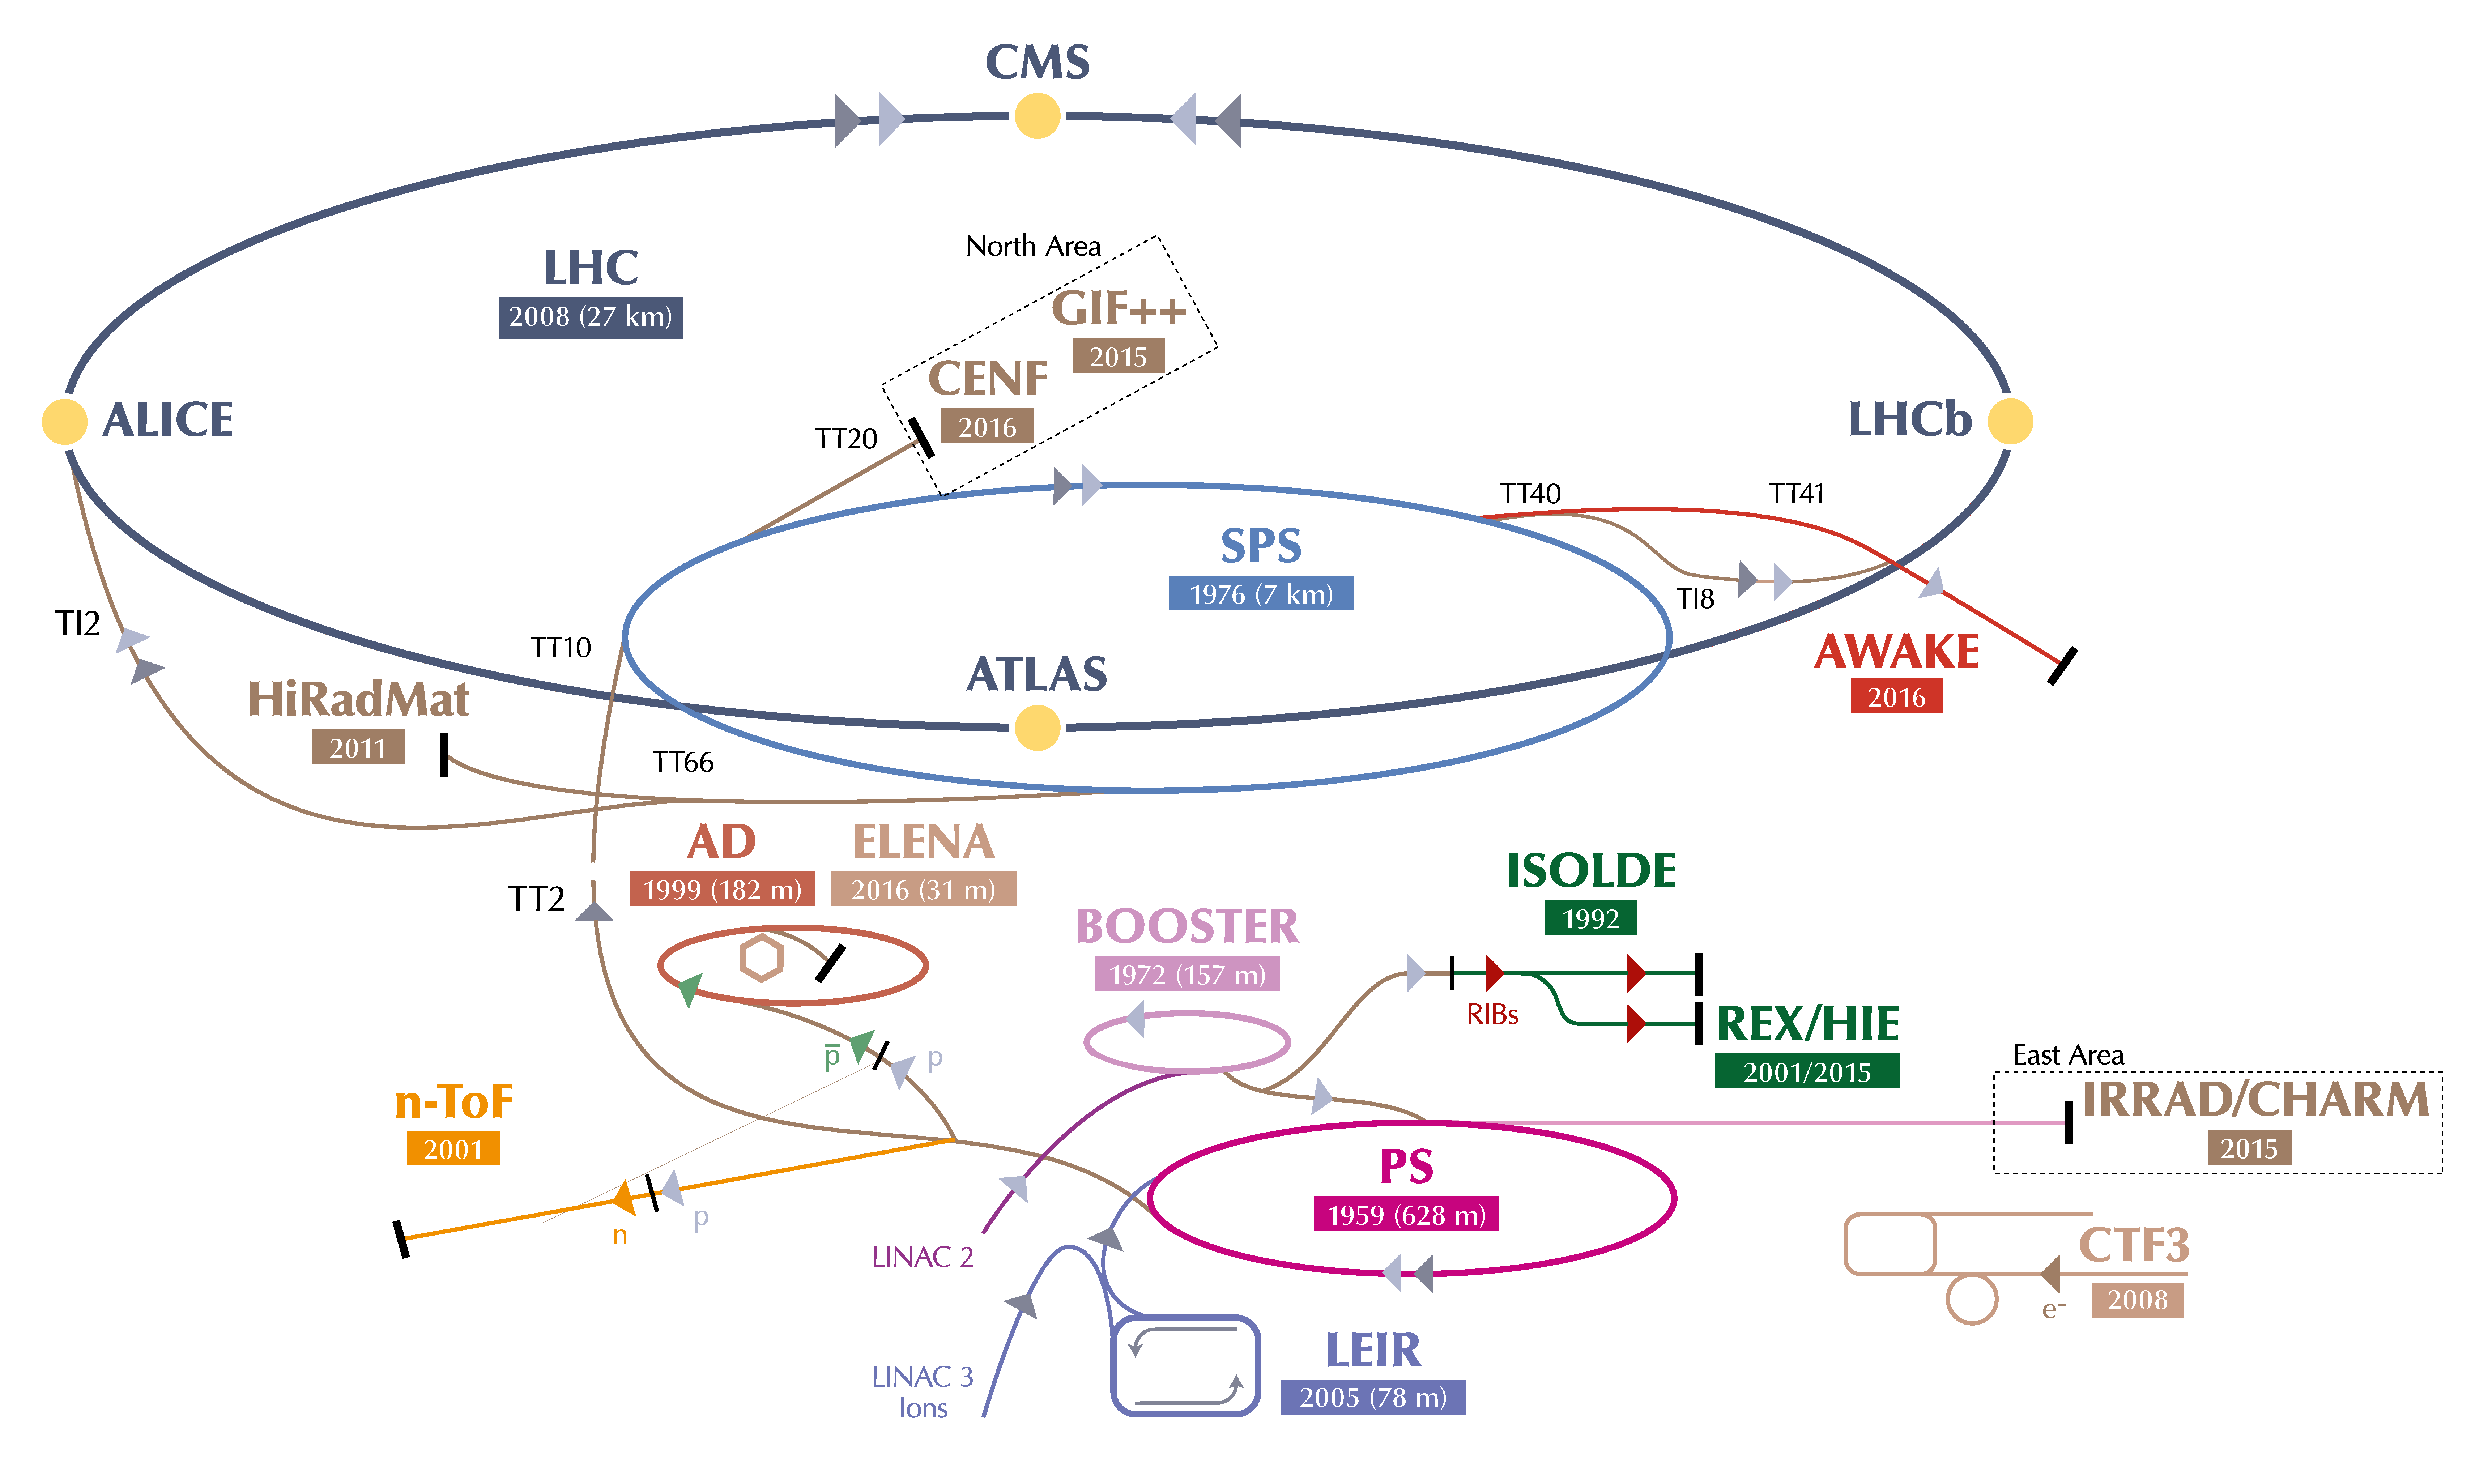
\includegraphics[width=0.99\linewidth,trim={20mm 0mm 20mm 0mm},clip]{figures/AcceleratorComplex}
    \caption{\label{Fig:WFA:AccComp} An overview of the CERN Accelerator Complex \cite{add:mobs:2016}.}
\end{figure}



Intro paper \cite{caldwell:2009}

Launch paper \cite{awake_collaboration:2014}

Evolution paper \cite{caldwell:2016}

Technical specs including simulation parameters \cite{gschwendtner:2016}


% ================================================================================================ %
\section{Evolution of the Concept}
\label{WFA:History}

Previous experiments, SLAC, etc.

\cite{rosenzweig:1988, blumenfeld:2007, kallos:2008, litos:2014}

Self modulation at FACET \cite{adli:2016}

Review by Patric \cite{muggli:2009}

% ================================================================================================ %
\section{AWAKE: A Design Overview}
\label{WFA:Design}

AWAKE is, as of the writing of this thesis, in Run 1. At the end of the proton beam line from the SPS, a $10\unit{m}$ plasma stage has been installed, with the laser needed to ionise the vapour. In addition, an electron source has been installed, and a new side tunnel had to be dug to fit the electron beam line connecting the source to the main assembly.

\begin{figure}[hbt]
    \centering
    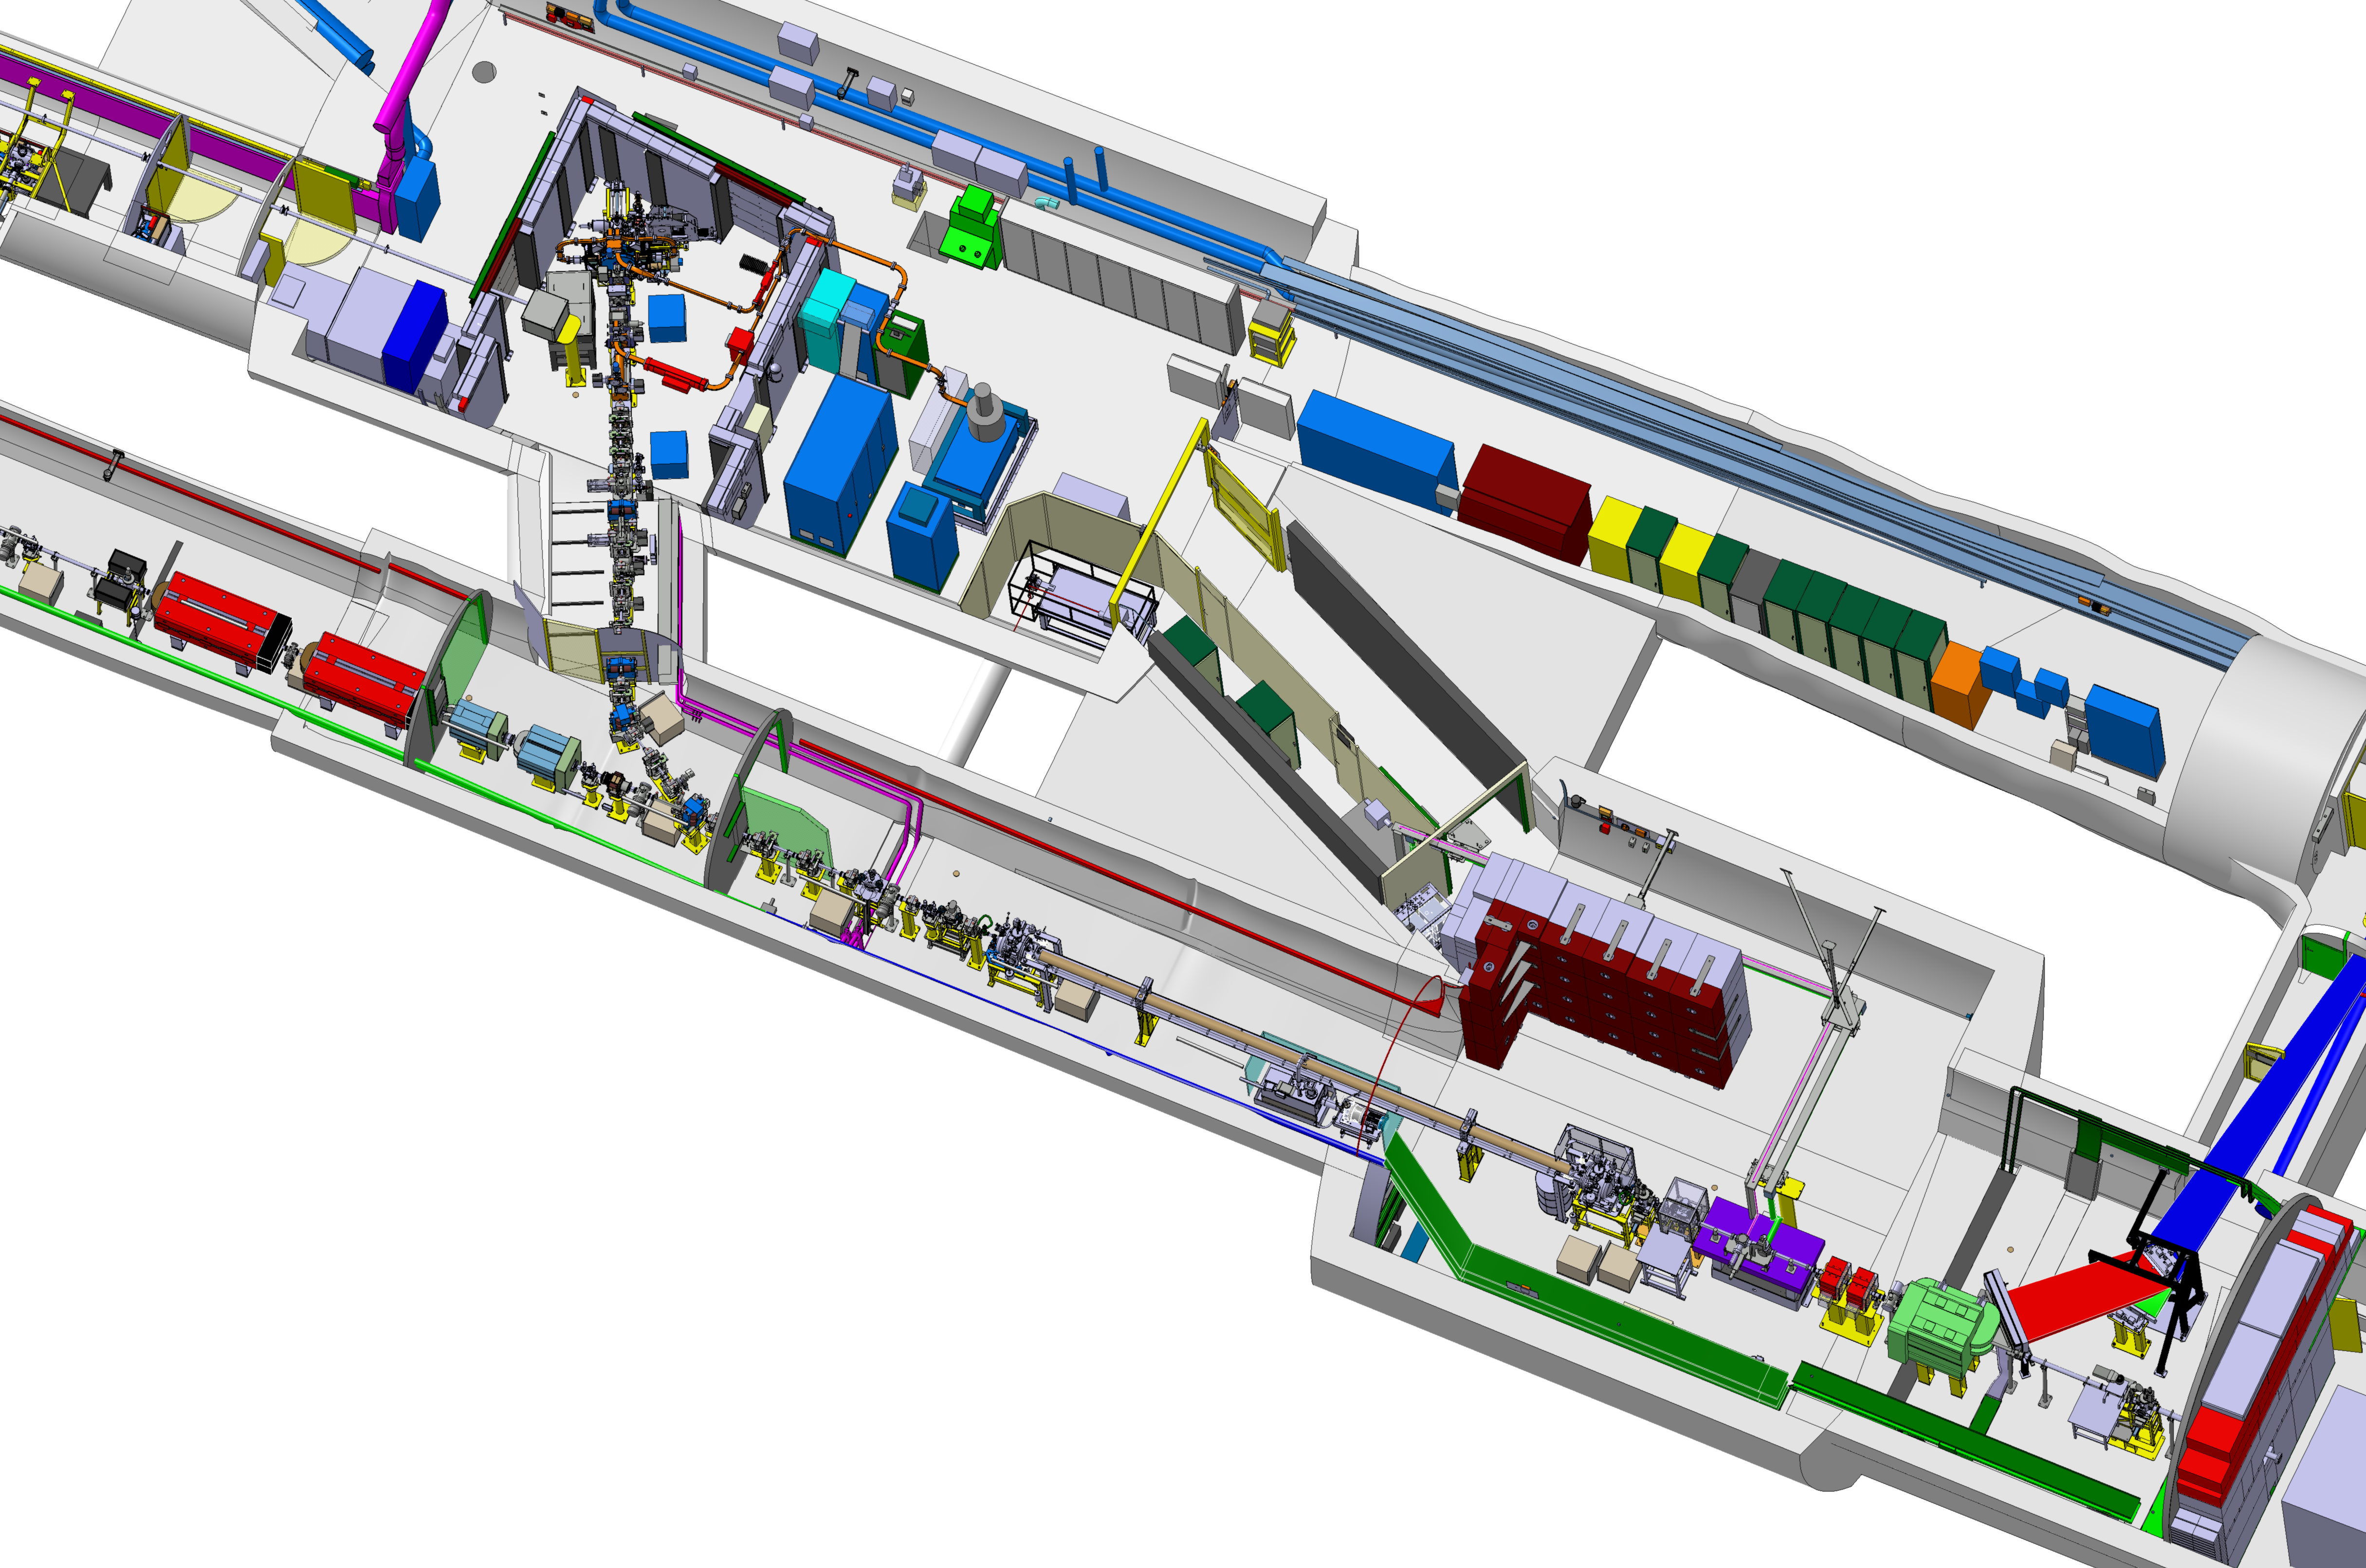
\includegraphics[width=0.99\linewidth,trim={0mm 0mm 0mm 0mm},clip]{figures/AwakeExperiment}
    \caption{\label{Fig:WFA:AWAKE} A CAD drawing of the AWAKE experimental area.}
\end{figure}

% ================================================================================================ %
\subsection{Plasma Source}
\label{WFA:Design:Plasma}

As per the 2015 Status Report, the requirements for the plasma source for AWAKE is a $10\unit{m}$ long cell with a plasma electron density of $1-10\nexp{14}\unit{cm}^{-3}$. The density variation should be within $0.2\%$, and the radius of the plasma channel should be $\geq 1\unit{mm}$. The plasma should also consist of heavy ions to mitigate ion motion \cite{caldwell:2015}.

\begin{figure}[hbt]
    \centering
    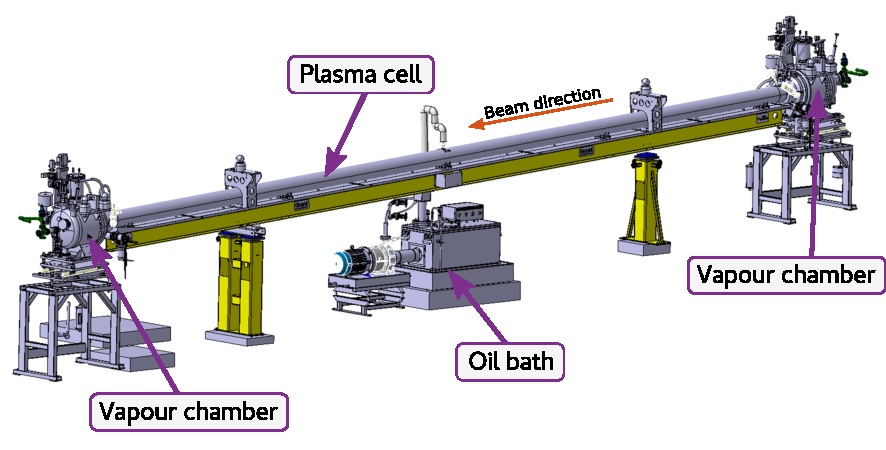
\includegraphics[width=0.99\linewidth,trim={0mm 0mm 0mm 0mm},clip]{figures/PlasmaCell}
    \caption{\label{Fig:WFA:PlasmaCell} A CAD drawing of the plasma cell and its related components, as presented in the 2016 AWAKE Status Report \cite{awake_collaboration:2016}.}
\end{figure}

For the AWAKE vapour source, rubidium (Rb) was chosen. Rubidium has a low melting point, $39.3\celsius$; a low first ionisation energy, $4.18\unit{eV}$; and a standard atomic weight of $85.47$. The plasma wavelength of rubidium ions with a $+1$ charge is roughly $400$ times that of the plasma electrons (see Eq. \ref{EQ:PWFA:L0W0}). An additional benefit of using an alkaline metal like rubidium is that the second ionisation level is significantly higher, $27.3\unit{eV}$, preventing a high risk of further ionisation and thus a lower charge/mass ratio. The rubidium vapour is created by heating the reservoir and the plasma cell to around $150-200\celsius$ to reach the density range required for AWAKE \cite{caldwell:2015}.

The ionisation of the Rb vapour is achieved with a short laser pulse co-propagating with the proton drive beam. In order to seed the self-modulation of the driver, the laser can be timed such that the plasma channel is created inside the beam itself.

% ================================================================================================ %
\section{Stages of the Experiment}
\label{WFA:AWAKE}

A summary of the AWAKE experiment

% ================================================================================================ %
\subsection{AWAKE Run 1}
\label{WFA:AWAKE:R1}

\begin{table}[hbt]
    \centering
    \caption{Nominal AWAKE experiment beam parameters for Run 1 \cite{gschwendtner:2014, gschwendtner:2016}.}
    \label{T:AWAKE-Run1}
    \begin{tabular}{lll}
        \hline
        \textbf{Parameter} & \textbf{Proton Beam} & \textbf{Electron Beam} \\
        \hline
        Momentum &
            $400\unit{GeV}$               & $16\unit{MeV}$ \\
        Charge &
            $4.8\unit{nC}$                & $200\unit{pC}$ \\
        Particles &
            $3\nexp{11}$                  & $1.25\nexp{9}$ \\
        Bunch length ($\sigma_{z}$) &
            $12\unit{cm}\;(0.4\unit{ns})$ & $1.2\unit{mm}\;(4\unit{ps})$ \\
        Bunch size ($\sigma_{x,y}$) &
            $200\unit{\mu m}$             & $250\unit{\mu m}$ \\
        Normalised emittance ($\emitN$) &
            $3.5\unit{\mu m}$             & $2\unit{\mu m}$ \\
        Relative energy spread ($\Delta p/p$) &
            $0.035\%$                     & $0.5\%$ \\
        Beta function ($\beta^{*}_{x,y}$) &
            $4.9\unit{m}$                 & $0.4\unit{m}$ \\
        Dispersion ($D^{*}_{x,y}$) &
            $0$                           & $0$ \\
        \hline
    \end{tabular}
\end{table}

Description of Run 1. SMI, long e-beam.

% ================================================================================================ %
\subsection{AWAKE Run 2}
\label{WFA:AWAKE:R2}

Short e-beam, multiple stages, etc.

Problems relevant for this thesis.

Erik \cite{adli:2016a}

% ================================================================================================ %
\section{The Self-modulation Instability in AWAKE}
\label{WFA:SMI}

Results from Run 1 of the experiment.

% ================================================================================================ %
